Considere las ruedas dentadas $A$ y $B$, de la transmisión de una bicicleta (véase Figura de este problema). Como se sabe, el engrane $B$ está unido a la rueda trasera $C$, y gira junto con ella cuando el ciclista pedalea. Suponiendo que lo anterior está ocurriendo, diga si:
\begin{enumerate}
    \item La velocidad lineal de un punto en la periferia de $A$, es mayor, menor o igual que la de un punto en la periferia de $B$.
    \item La velocidad angular de A es mayor, menor o igual que la velocidad angular de $B$.
    \item La velocidad angular de $B$ es mayor, menor o igual que la velocidad angular de $C$.
    \item La velocidad lineal de un punto en la periferia de $B$, es mayor, menor o igual que la de un punto en la periferia de $C$.
\end{enumerate}
\begin{figure}[h!]
  \centering
  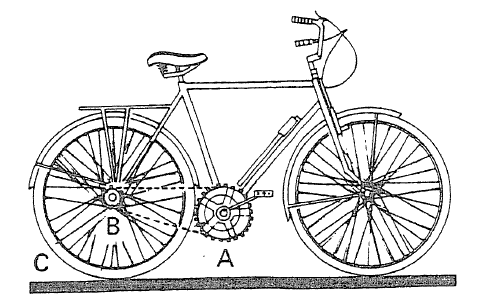
\includegraphics[scale=0.45]{figuras/fig_alvarenga_p134_19.png}
  \caption{Problema 3}
\end{figure}